% A skeleton file for producing Computer Engineering reports
% https://kgcoe-git.rit.edu/jgm6496/KGCOEReport_template

\documentclass[CMPE]{KGCOEReport}

% The following should be changed to represent your personal information
\newcommand{\classCode}{CMPE 663}  % 4 char code with number
\newcommand{\name}{Andrei Tumbar}
\newcommand{\LabSectionNum}{1}
\newcommand{\LabInstructor}{Wolfe}
\newcommand{\TAs}{Nitin Borhade}
\newcommand{\exerciseNumber}{3}
\newcommand{\exerciseDescription}{Bank}

\usepackage{tikz}
\usepackage{circuitikz}
\usetikzlibrary{calc}
\usepackage{multirow}
\usepackage{titlesec}
\usepackage{float}
\usepackage{lmodern}
\usepackage{siunitx}
\usepackage{subcaption}
\usepackage{graphicx}
\usepackage[usestackEOL]{stackengine}
\usepackage{scalerel}
\usepackage[T1]{fontenc}
\usepackage{amsmath}


\def\code#1{\texttt{#1}}

\begin{document}
    \maketitle
    \section*{Analysis/Design}

    This project looked at implementing a simulated bank using the
    features provided by FreeRTOS. The bank was simulated by providing
    accurate and scaled timings for transactions between customers and
    bank tellers. Random variables that drove the probabilities of certain
    actions were generated using the hardware RNG over a uniform distrobution
    across given boundaries. \\

	\subsection*{Simulation}

	The design of the bank involved four main tasks in addition to two status
	tasks. Each teller is given its own RTOS task and they are all waiting on
	the same queue. FreeRTOS's scheduler works by scheduling the task with the
	highest priority that is ready to execute. If multiple ready tasks have the
	same priority, the scheduler will alternate between them. This means that if
	multiple tasks with the same priority are to block due to a queue, the task
	that has not been serviced over the longest time interval will be scheduled
	next. In other words, the teller that has not seen a client for the longest
	time, will be given priority to pick from the queue. This allows a fair
	distrobution of customers to each of the three tellers.\\

	The fourth task running on the RTOS involves adding customers to the queue.
	It will generate a customer in a random time interval and queue the customer.
	When the work day is up, this task will self suspend.

	\subsection*{Metrics}

	An important aspect of this project was to provide a mechanism for reporting
	simulation metrics at the end of the work day. Because all metrics could be
	fit into either a maximum, minimum, or arithmetic average, a \code{Statistic}
	data structure was created to model any metric that was asked for. During the
	relevant events, the teller or the customer creation tasks would report a metric
	which would in turn be added to its corresponding statistic structure. When
	reporting the totals at the end, averages could easily be calculated from the
	sum and count of the statistic and min/max were kept track of as each event was
	reported.

	\subsection*{Status}

	The two status tasks running at lower priority simply handle writing the
	current teller status to the uart and writing to the seven segment display.
	They are running at a lower priority for two reasons. First being that the
	simulation accuracy would be slightly impacted if they were running at the
	same priority as the tellers. Secondly, putting these tasks at a lower
	priority allows them to run during all of the idle time that the CPU had.
	This proved to be fast enough to provide accurate status while still
	maintaining accuracy.

	\subsection*{Grad-portion}

	The grad-portion of this assignment involved writing to the seven segment
	display. Because the seven segment display works by keeping a single command
	in its memory, each digit in the number had to be continously written to the
	display to get a proper reading. The task performing this action runs a constant
	loop absorbing as many cycles are possible to create a clear image.

    \section*{Test Plan}

    Testing the code was fairly straighforward. The UART status task was updated
    in realtime and therefore showed most of the errors on the spot. The uniform
    distrobution of the RNG could be verified by making sure the minimum and maximum
    were close to the specified boundaries as well as the average being halfway between
    the two. The seven segment display was tested using the given customer entry rates
    as well as increased rates designed to fill the queue more.

    \section*{Project Results}

    The software behaved as expected by the problem statement. All random numbers
    generated expected results and the simulation ran in the expected amount of
    time. The metrics reported at the end of the simulation showed that the parameters
    controlling the simulation as well as the design of the bank were correct.

    \section*{Lessons Learned}

	This project explored creating an embedded system on top of FreeRTOS. I learned
	how to use the API reference to quickly implement the components I needed in this
	realtime system. Task scheduling priority and preemption became clear when
	expirementing with task attributes during development. The most major issue that
	I ran into during development was a hardfault inside the teller. I created an
	efficient way to debug hardfaults (and other faults) by creating an assembly
	subroutine to extract the core registers saved when the hardfault interrupt was
	triggered. This allowed me to view the instruction and register values of the
	problematic code. The problematic code ended being related to a libc library call
	\code{vsnprintf} not being thread-safe and therefore causing issues within FreeRTOS.

	\pagebreak

	Below is an example of a hardfault occuring when overwriting part of the task
	control block (FreeRTOS's structure for keeping track of tasks) causing the
	context switcher to fault out:

	\begin{figure}[h!]
      \centering
      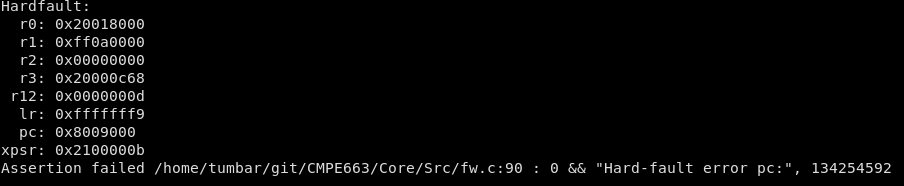
\includegraphics[width=5.5in]{hardfault}
      \caption{Example of hardfault handler}
      \label{fig:fault}
    \end{figure}

	Looking at the program counter in Figure \ref{fig:fault}, we can find the appropriate
	assembly instruction in the generated ELF binary. To do this, LLVM's objdump tool
	was used to decode the binary.

	\begin{figure}[h!]
      \centering
      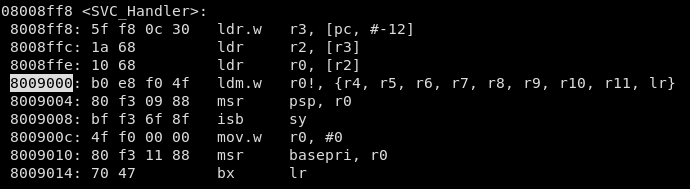
\includegraphics[width=5.5in]{fault_pc}
      \caption{Decoded instruction at faulty program counter}
      \label{fig:fault_pc}
    \end{figure}

\end{document}
